\subsection{تخمین پارامتر کانال رول}
برای اصلاح پارامترها رول چندین آزمایش انجام شد و با استفاده از خروجیآزمایش و جعبه‌ابزاز
\lr{Parameter Estimator}
پارامترها اصلاح شدند.
برای آزمایش رول هر یک از موتورهای دو و چهار  با دور مختلف شروع به حرکت کردند و خروجیسنسور داده برداری شد. سپس، مدل و پارامترهای داده برداری شده به جعبه‌ابزار
\lr{Parameter Estimator}
داده شد. نتایج آزمایش‌های کانال رول بعد از اصلاح پارامترها در شکل‌های
(\ref{roll_ps1}, \ref{roll_ps2}, \ref{roll_ps3}, \ref{roll_ps4}, \ref{roll_ps5})
آورده شده است.

\begin{figure}[H]
	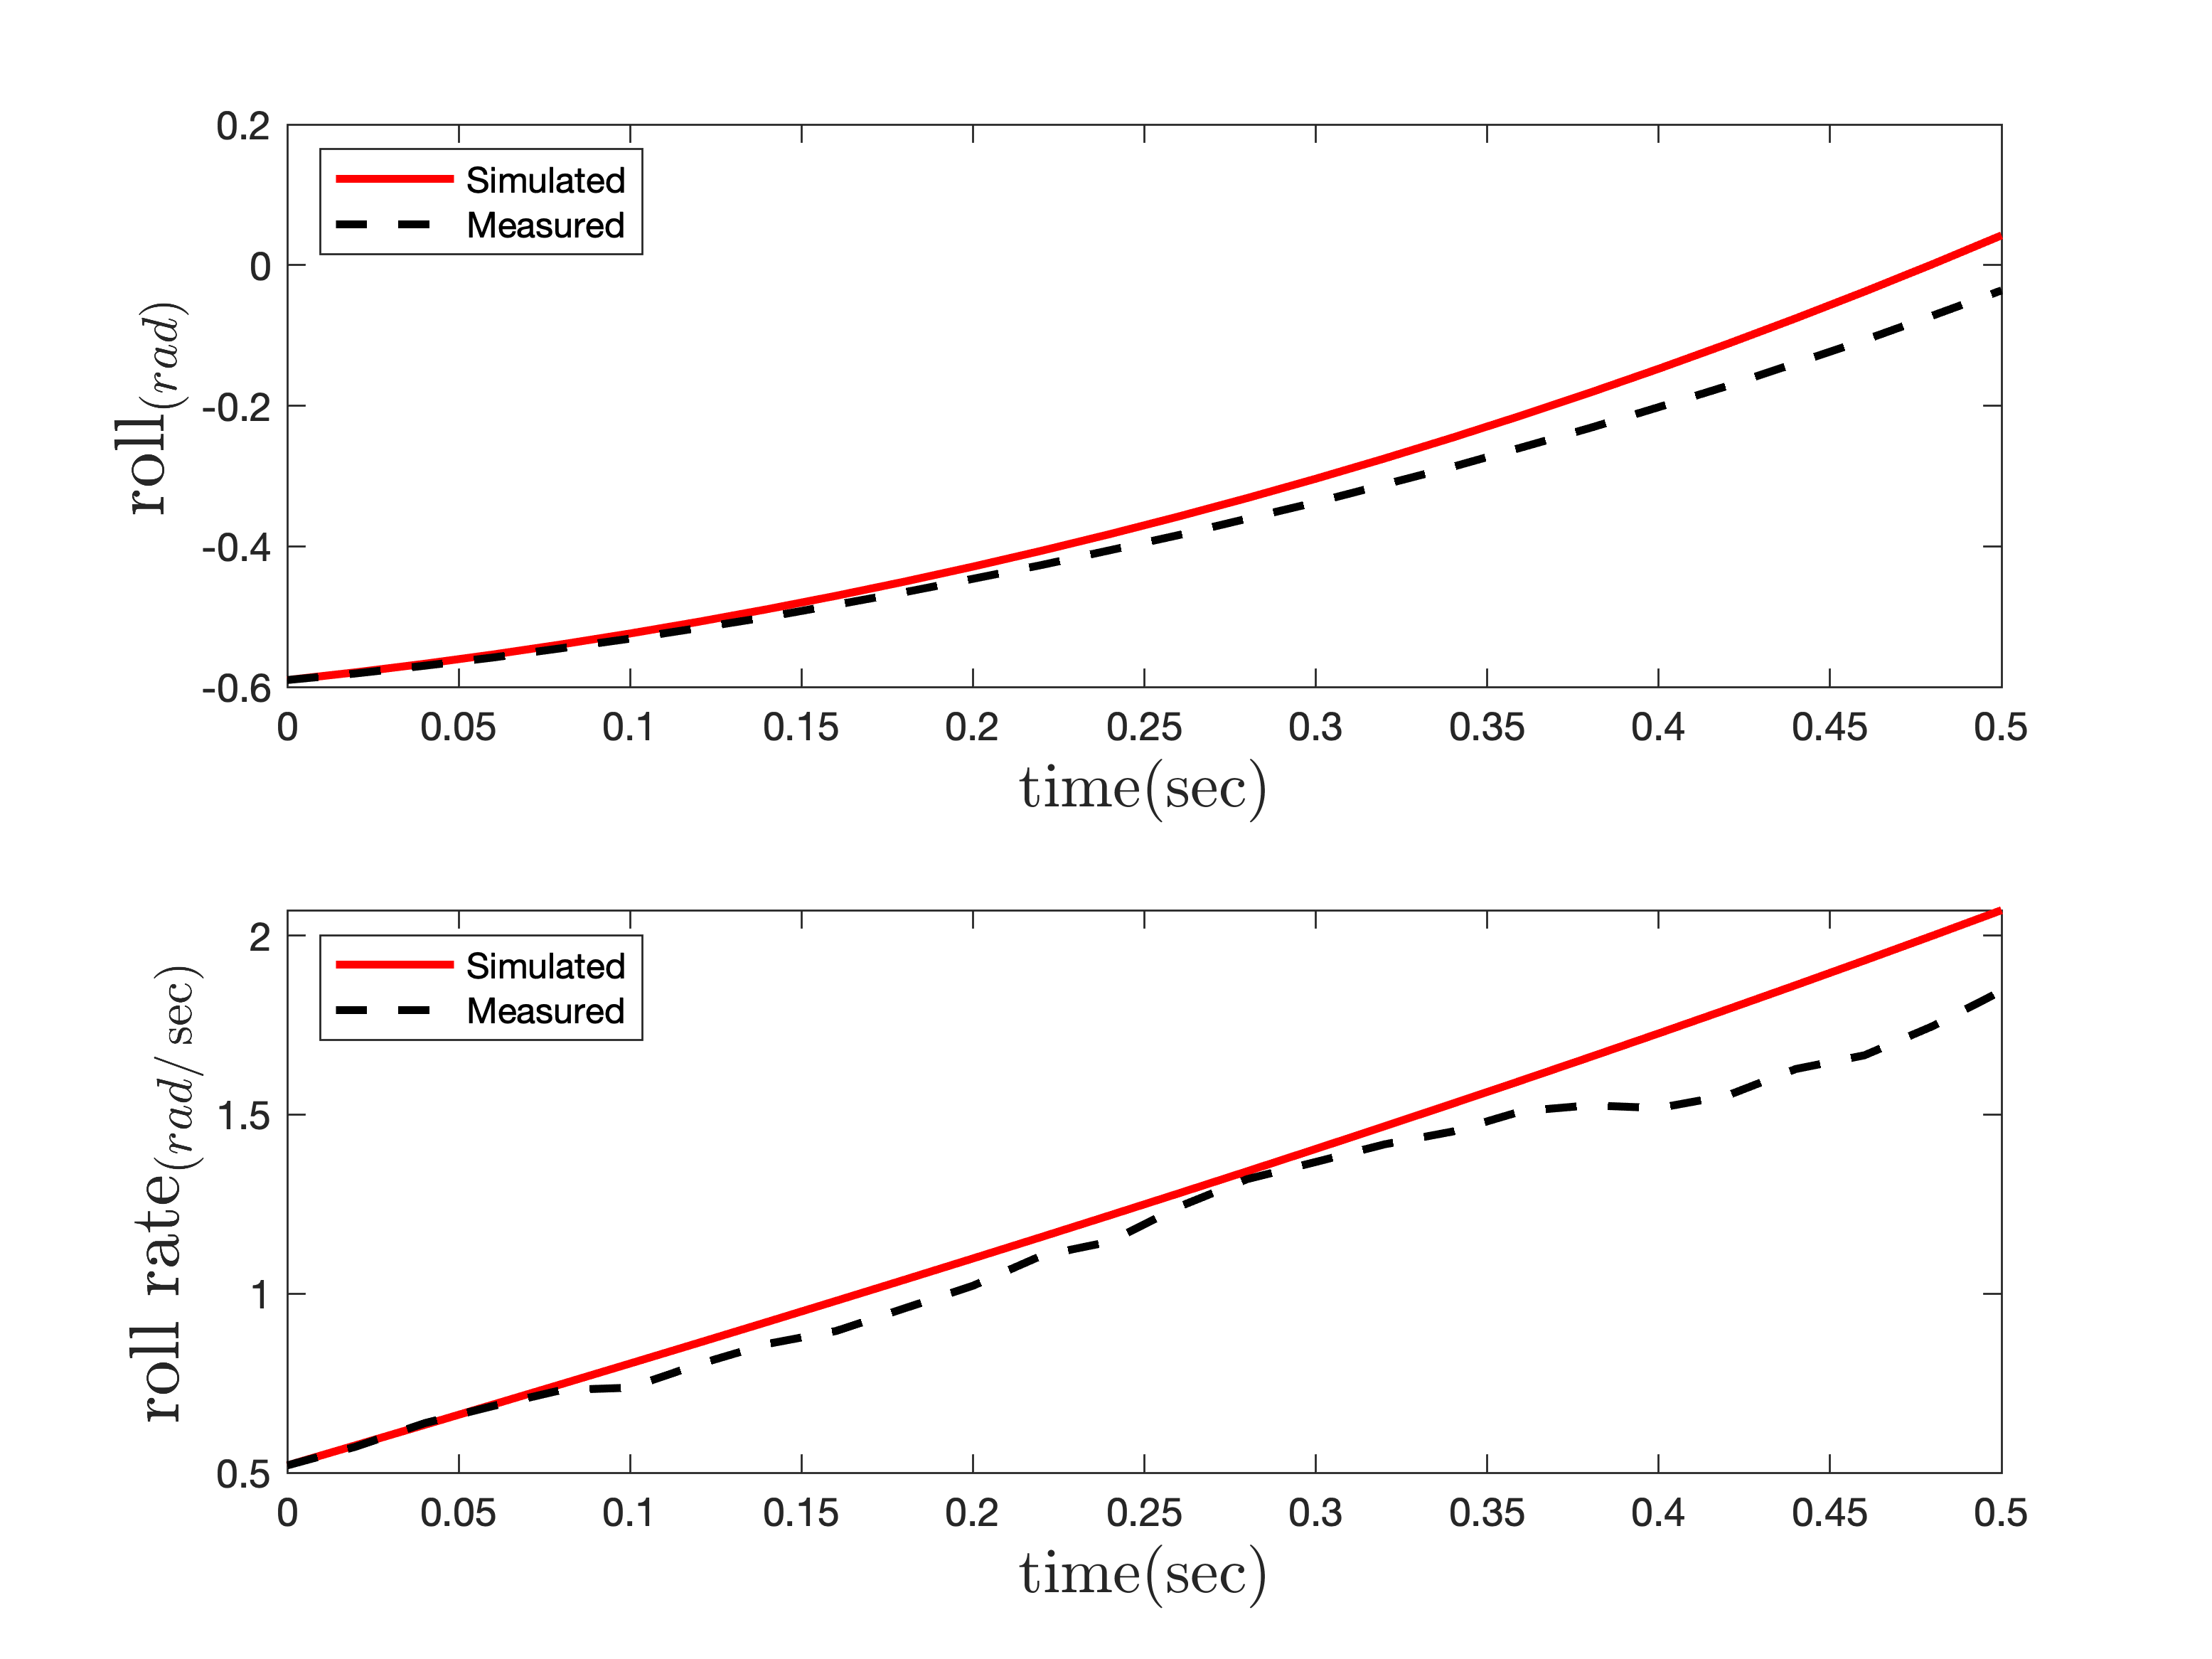
\includegraphics[width=12cm]{../../Figures/RCP/roll_parameter_estimation/RCP_roll_S1.png}
	\centering
	\caption{مقايسه خروجی‌های آزمايش اول و خروجیشبیه‌سازی پس از تخمین پارامترهای کانال رول}
	\label{roll_ps1}
\end{figure}
\begin{figure}[H]
	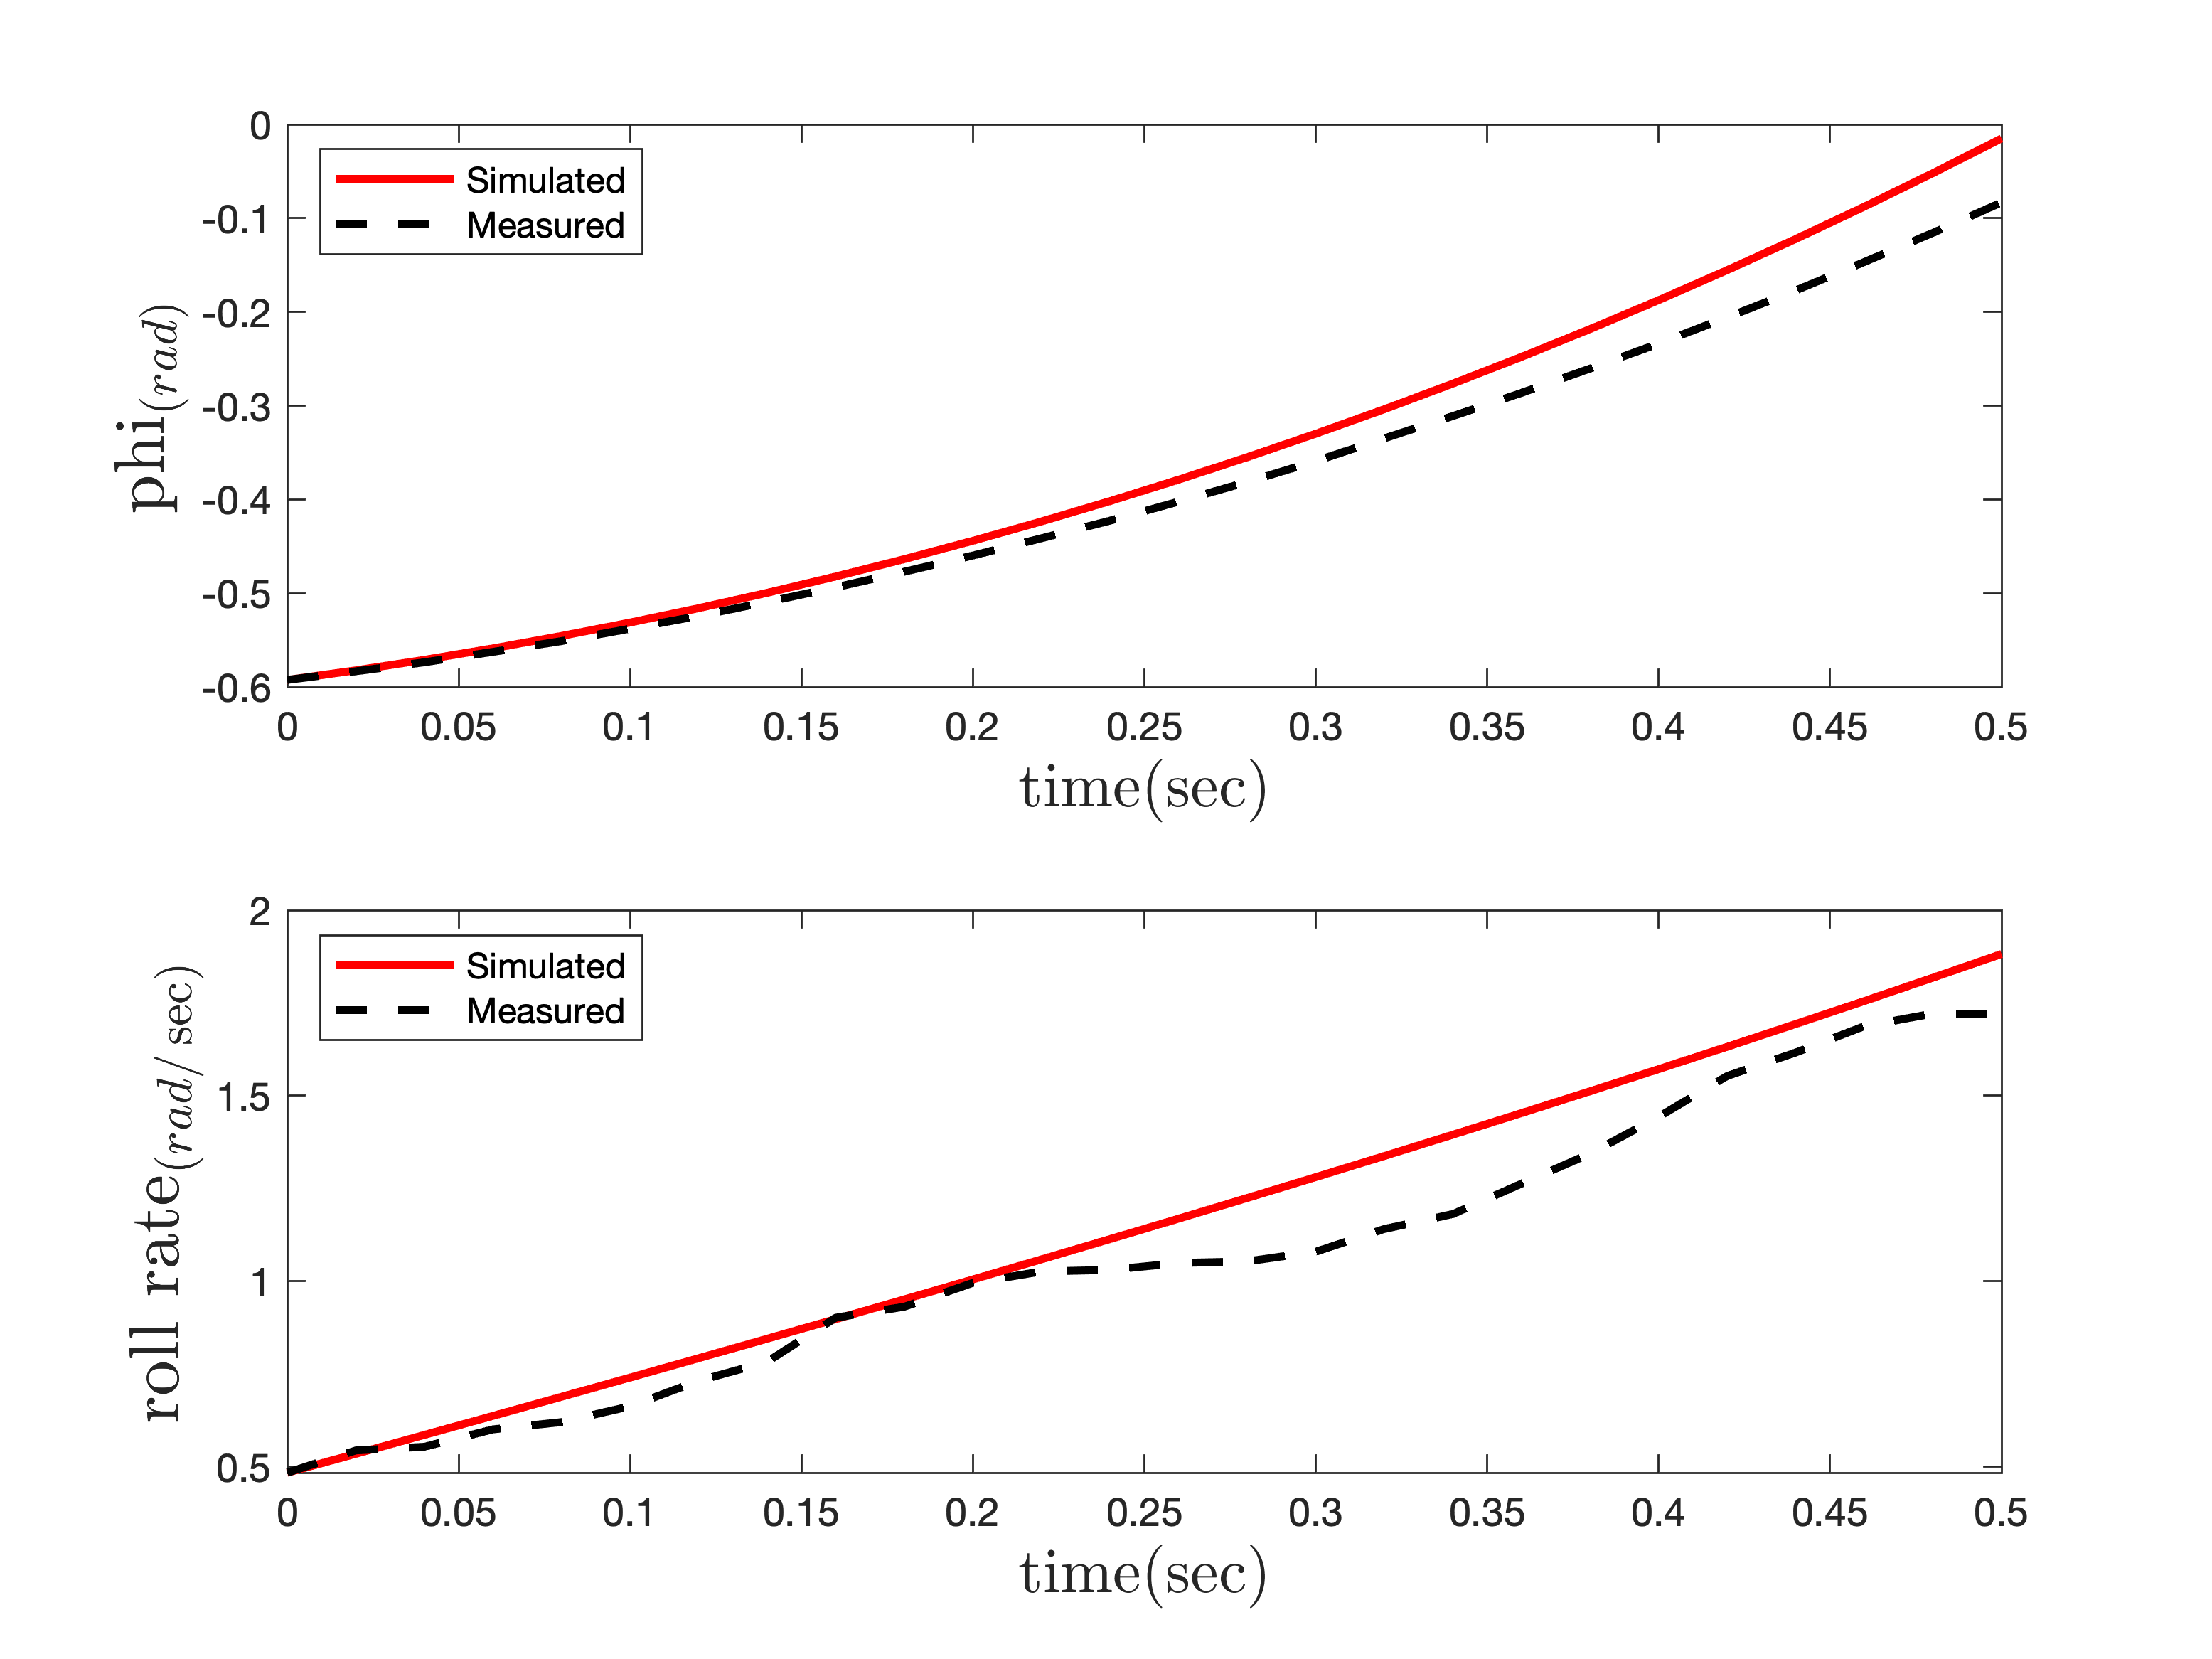
\includegraphics[width=12cm]{../../Figures/RCP/roll_parameter_estimation/RCP_roll_S2.png}
	\centering
	\caption{مقايسه خروجی‌های آزمايش دوم و خروجیشبیه‌سازی پس از تخمین پارامترهای کانال رول}
	\label{roll_ps2}
\end{figure}
\begin{figure}[H]
	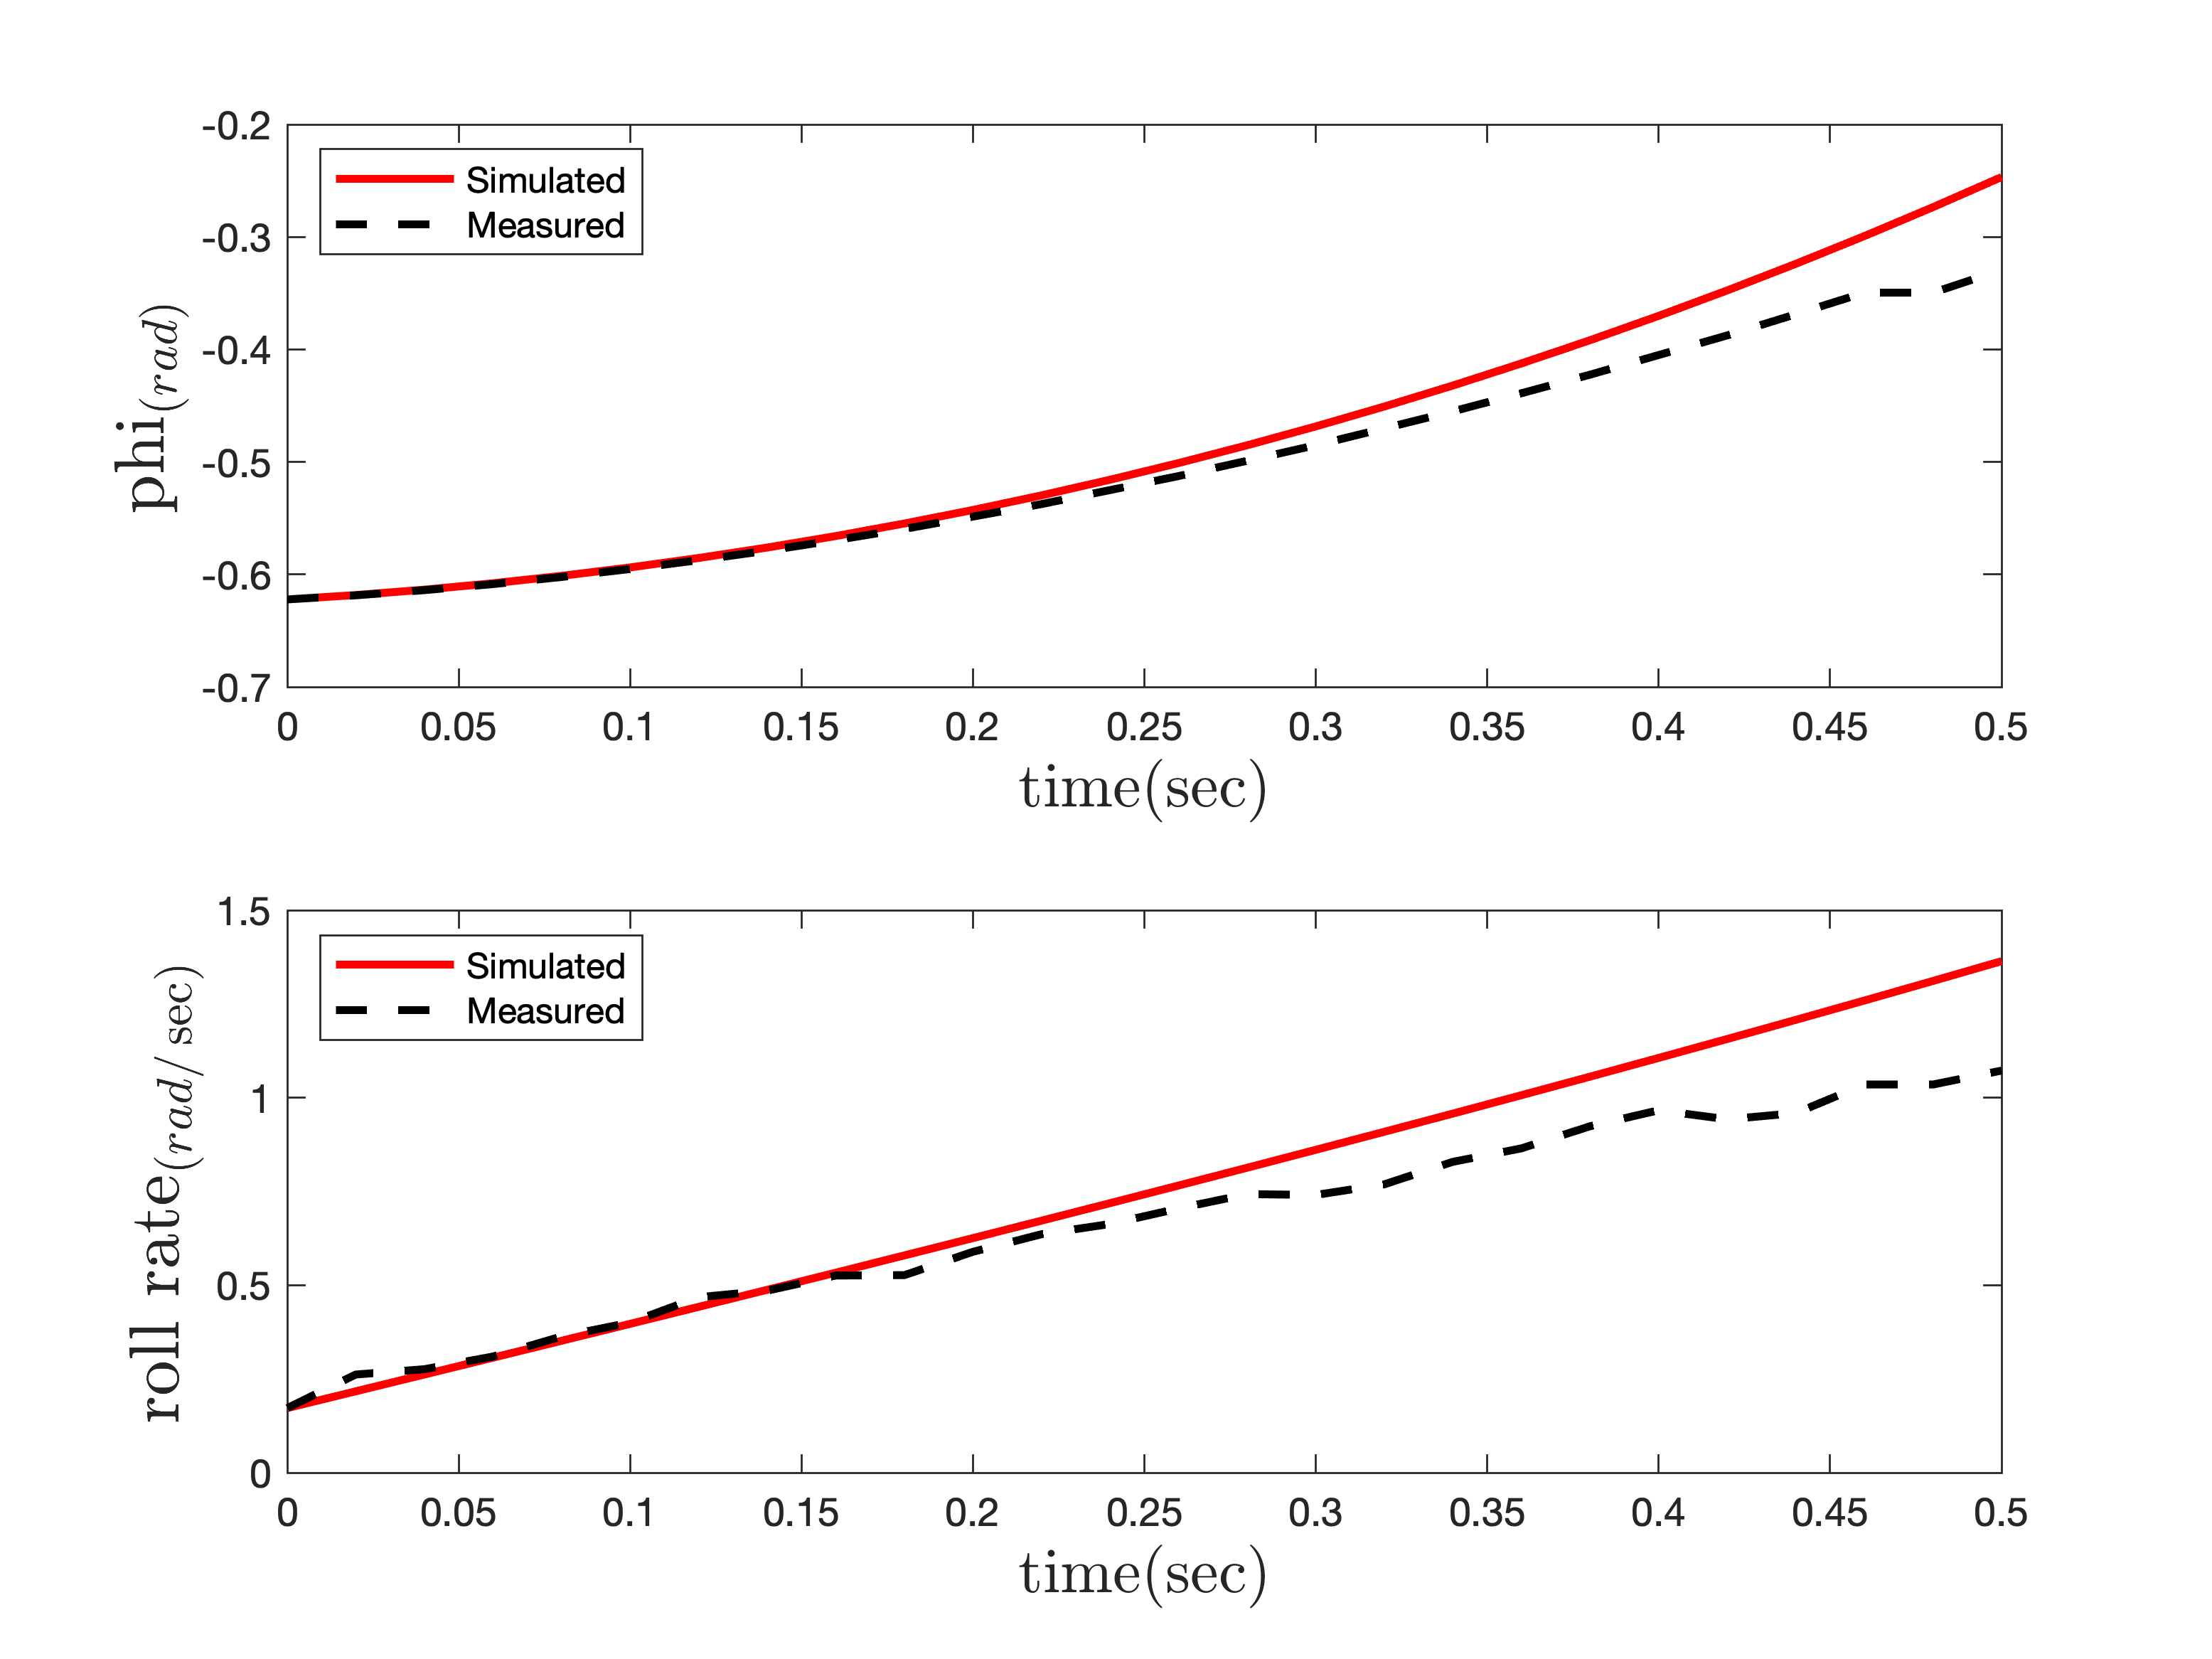
\includegraphics[width=12cm]{../../Figures/RCP/roll_parameter_estimation/RCP_roll_S3.png}
	\centering
	\caption{مقايسه خروجی‌های آزمايش سوم و خروجیشبیه‌سازی پس از تخمین پارامترهای کانال رول}
	\label{roll_ps3}
\end{figure}
\begin{figure}[H]
	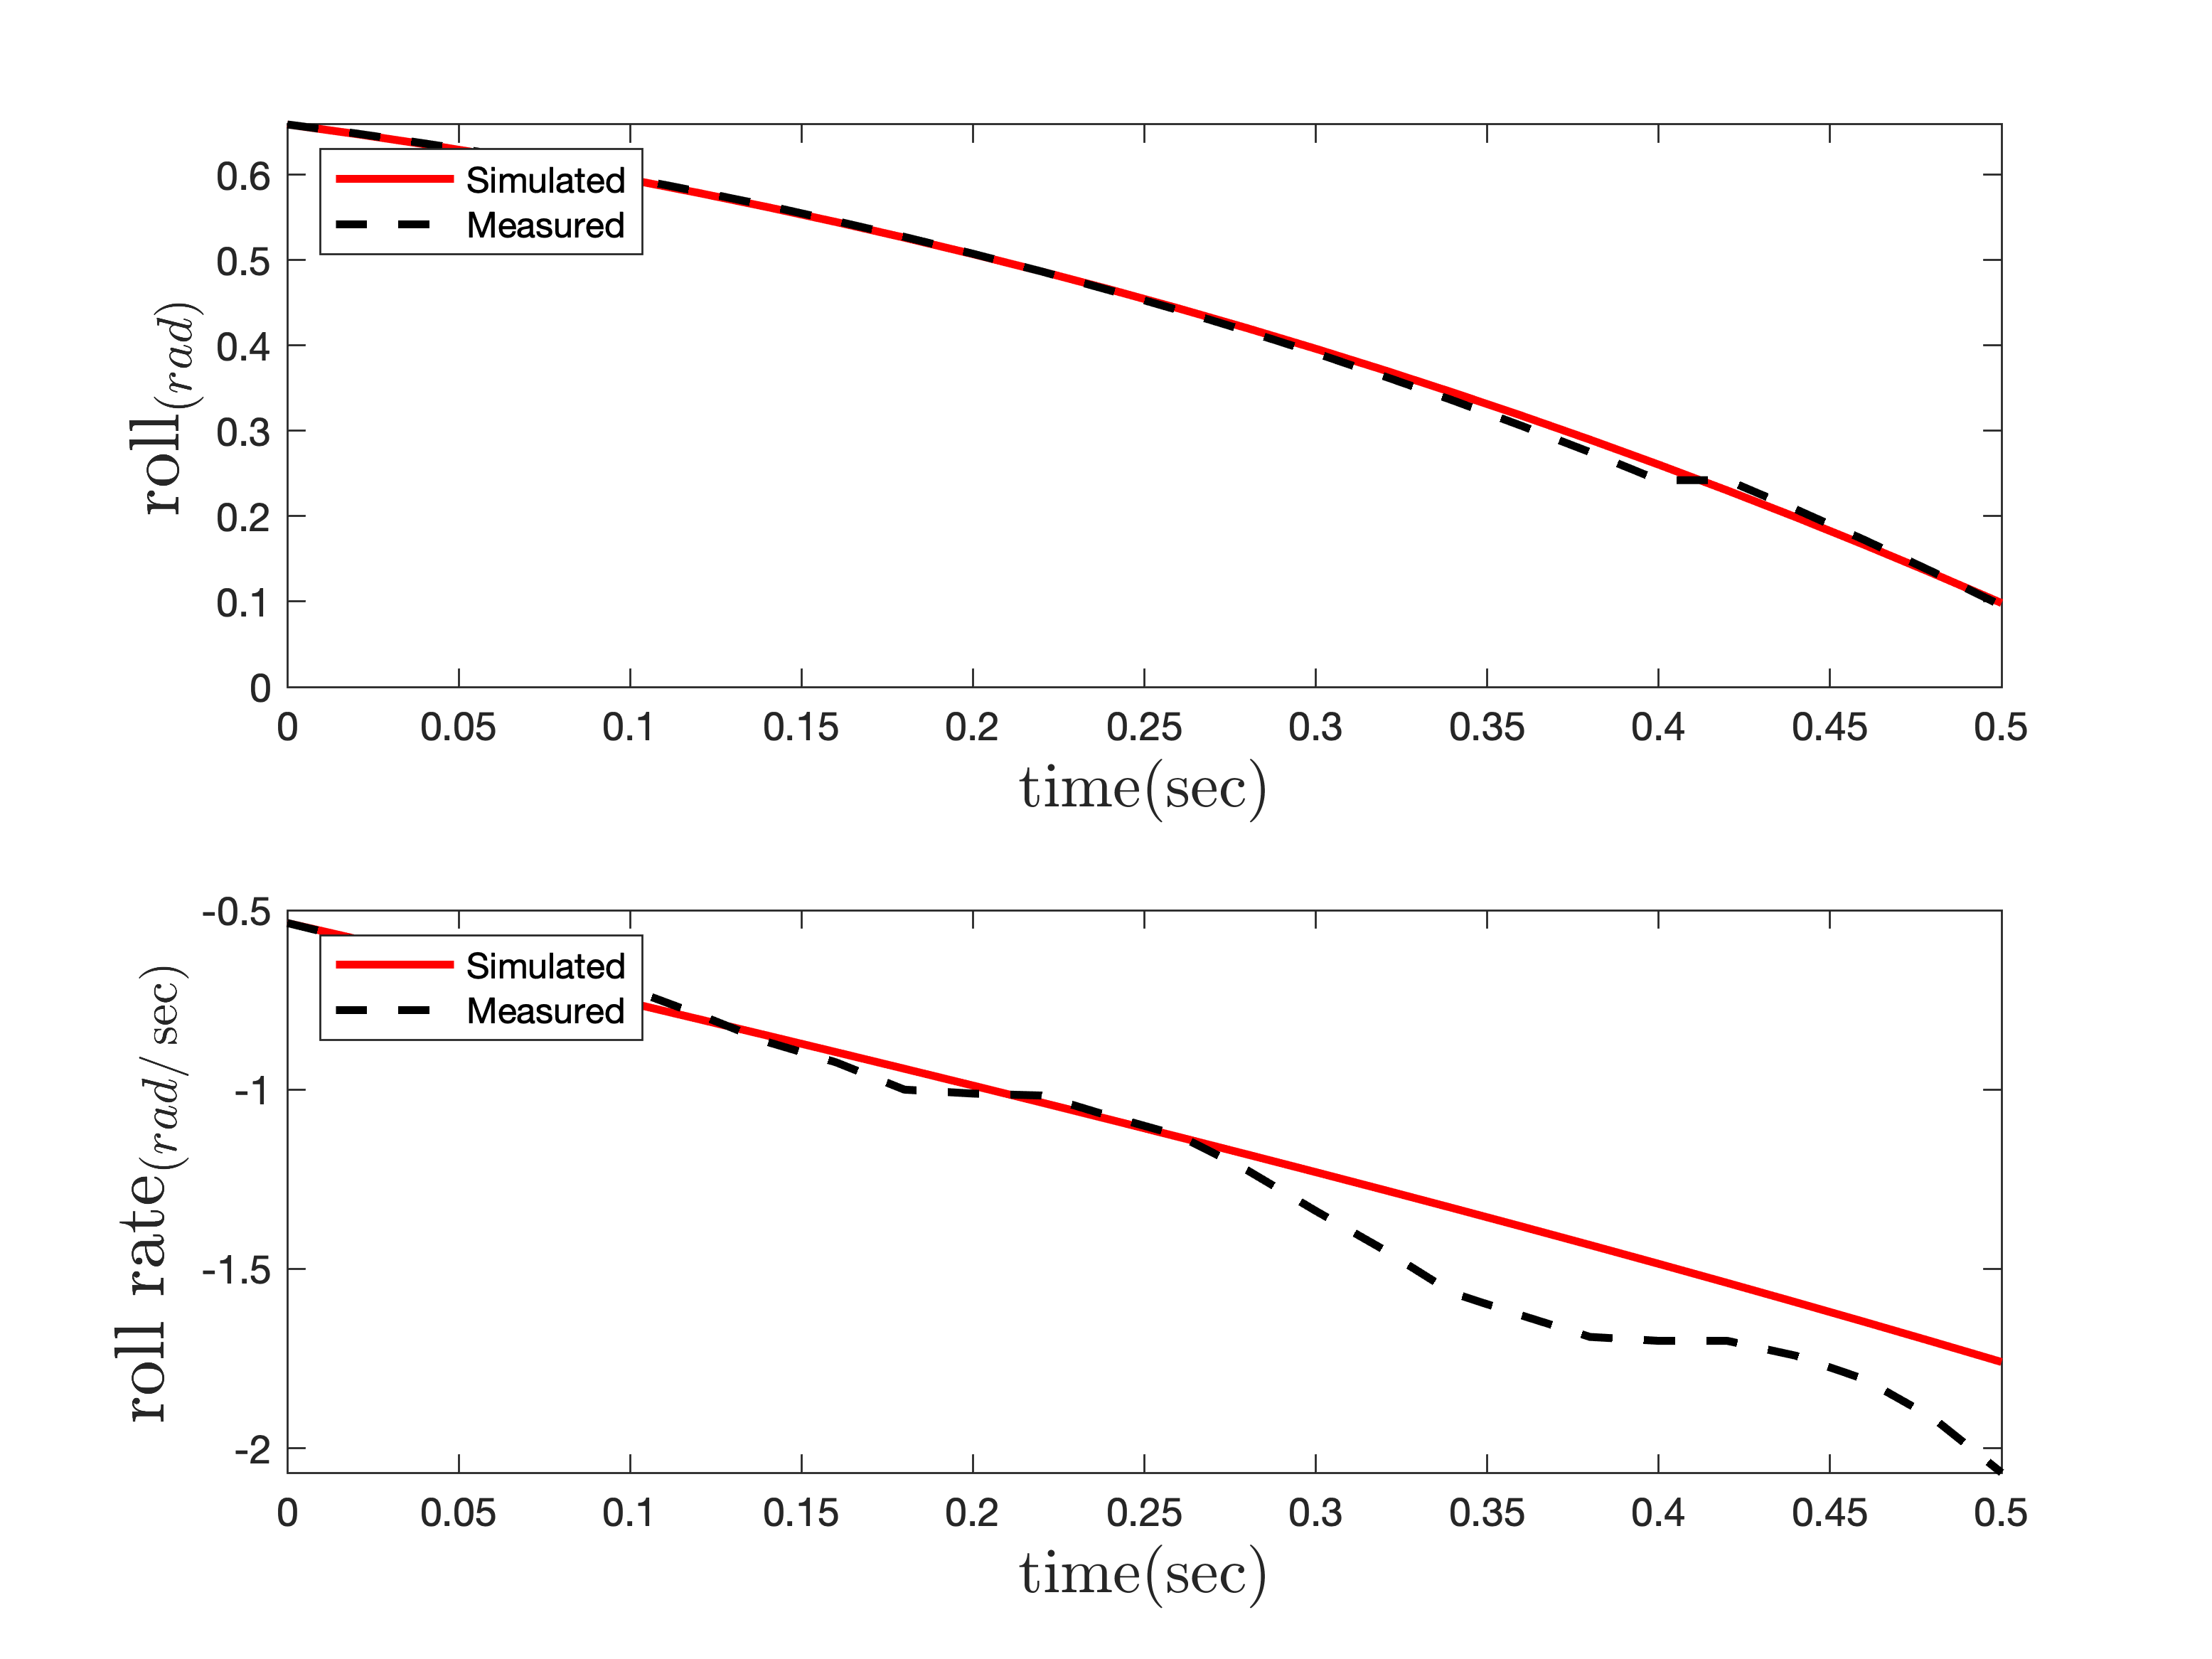
\includegraphics[width=12cm]{../../Figures/RCP/roll_parameter_estimation/RCP_roll_S4.png}
	\centering
	\caption{مقايسه خروجی‌های آزمايش چهارم و خروجیشبیه‌سازی پس از تخمین پارامترهای کانال رول}
	\label{roll_ps4}
\end{figure}
\begin{figure}[H]
	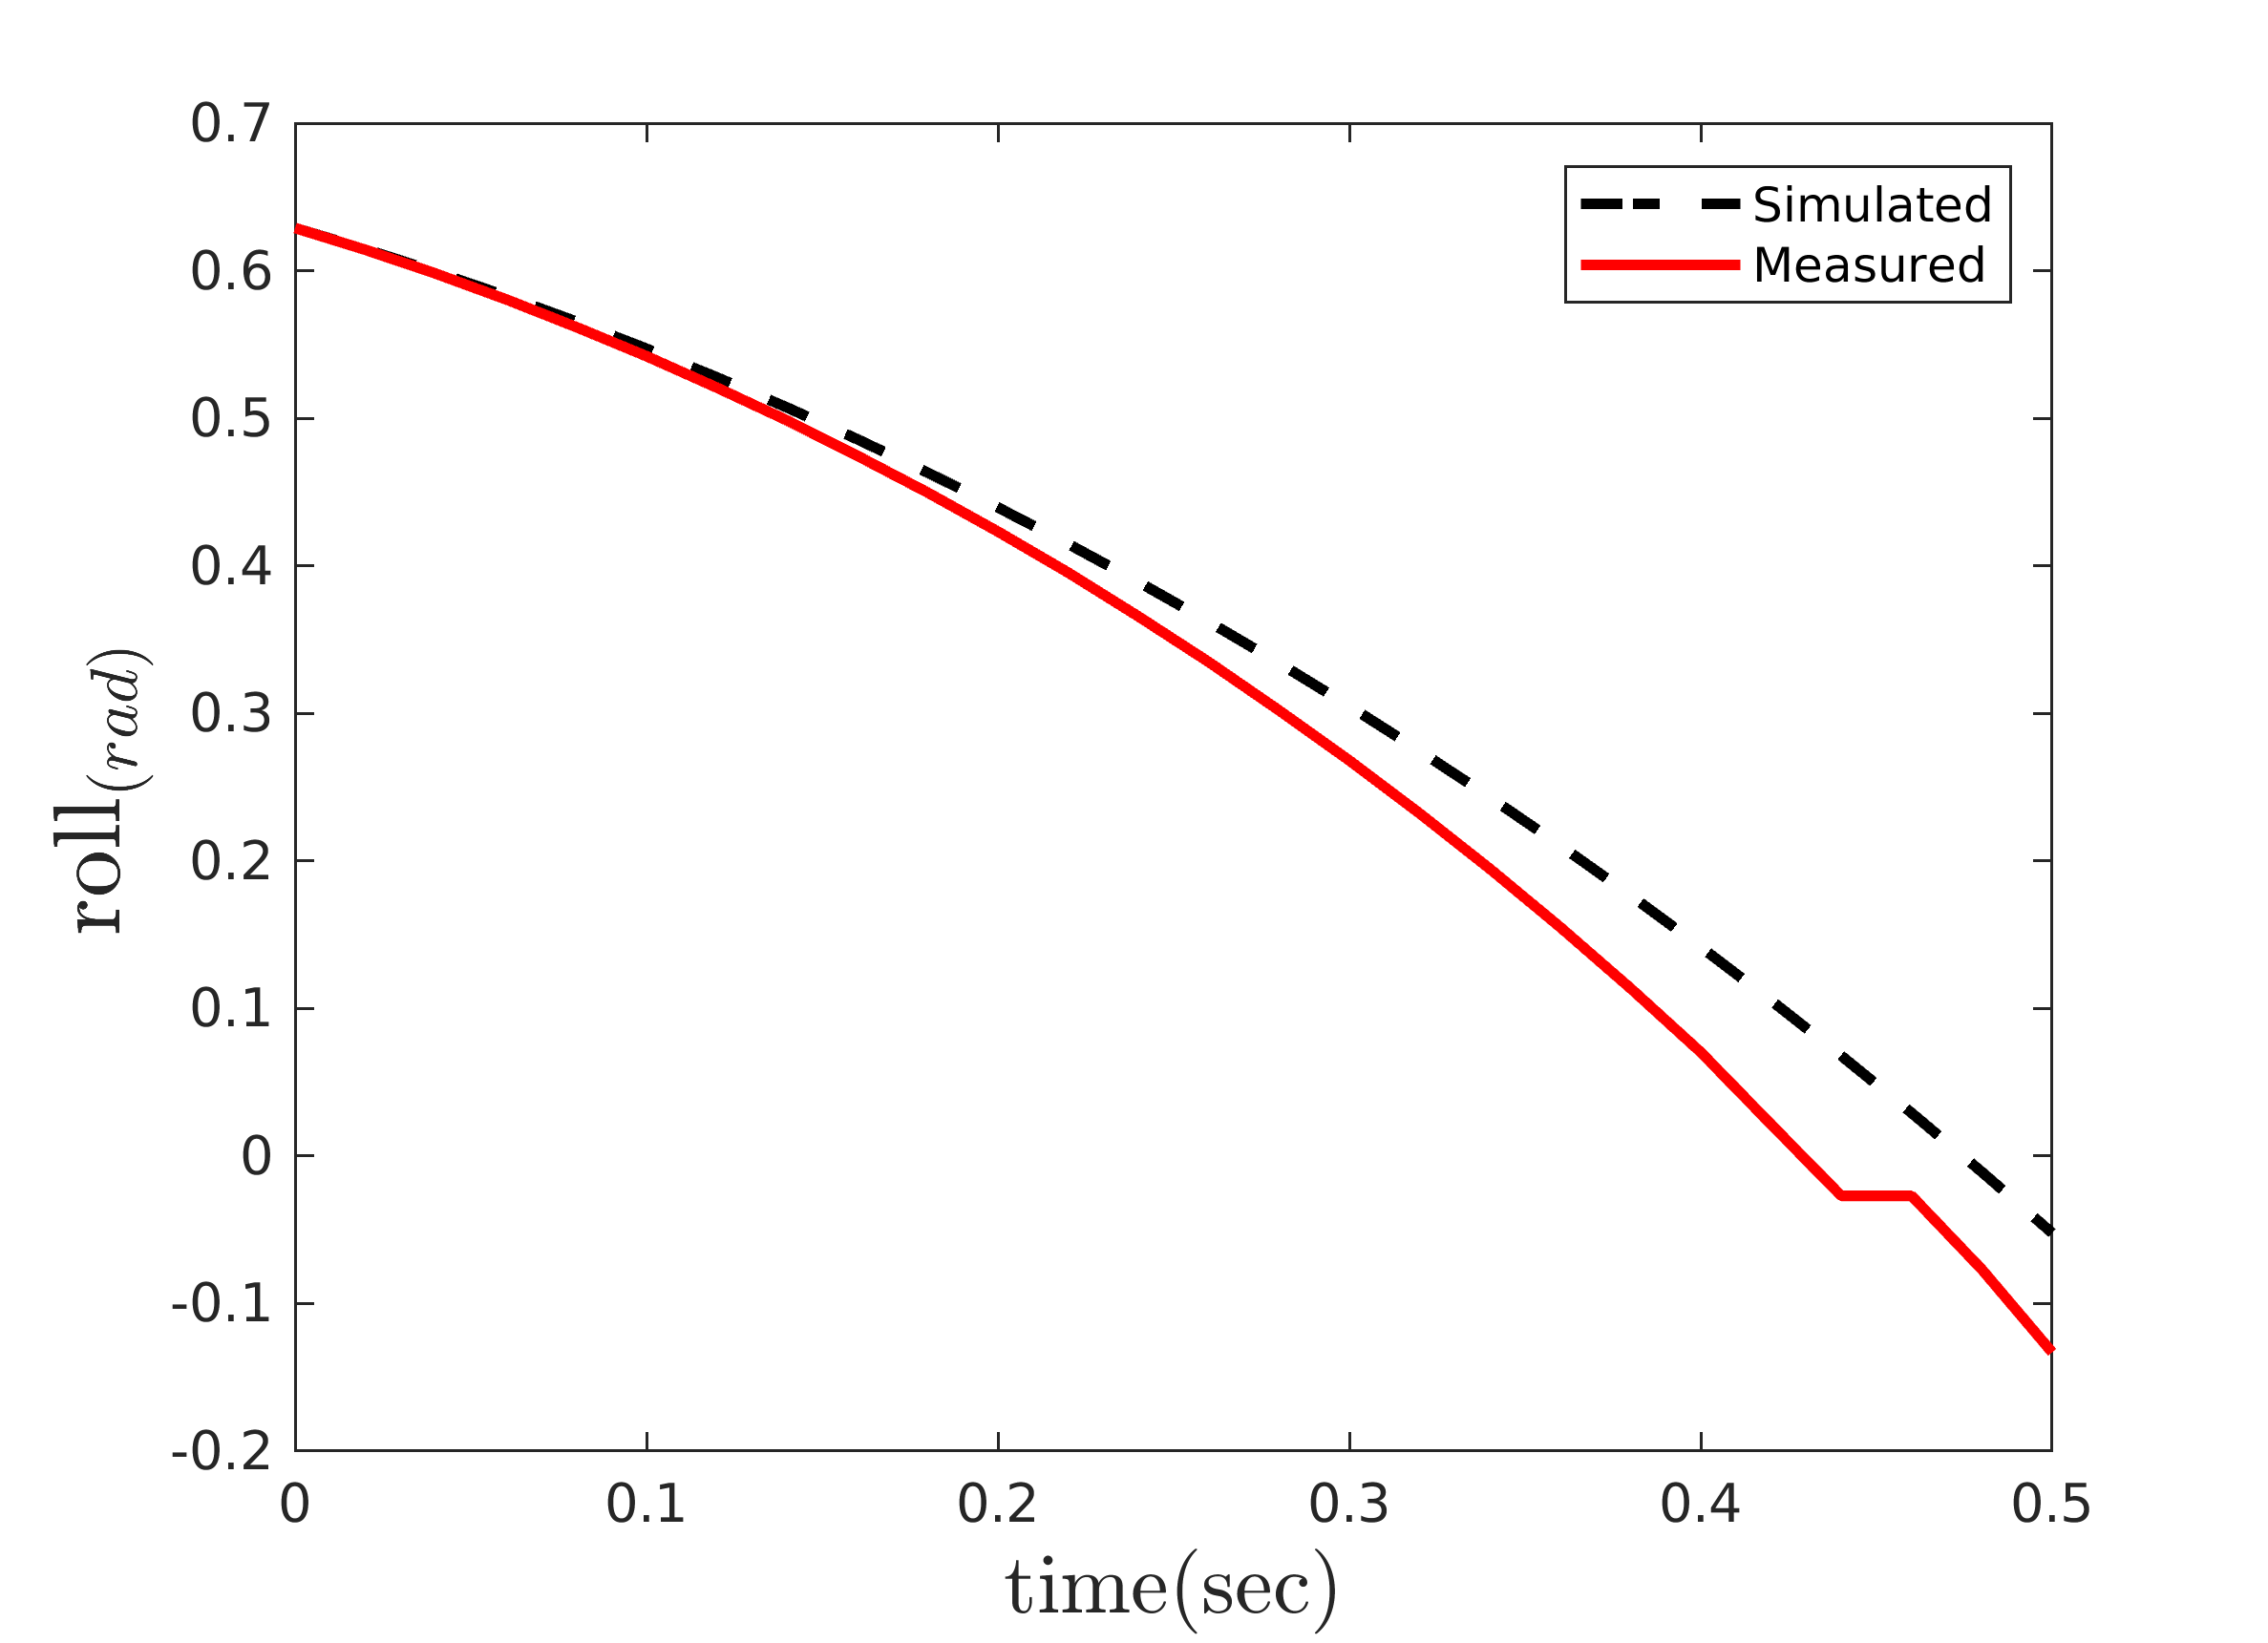
\includegraphics[width=12cm]{../../Figures/RCP/roll_parameter_estimation/RCP_roll_S5.png}
	\centering
	\caption{مقايسه خروجی‌های آزمايش پنجم و خروجیشبیه‌سازی پس از تخمین پارامترها کانال رول}
	\label{roll_ps5}
\end{figure}